\setcounter{secnumdepth}{3} %para tener una profundidad más en las enumeraciones
\chapter{Implementaci\'on}
\label{cap:implementacion}
En el Capítulo 3 se abordó la descripción de la herramienta sin entrar en detalles de como funcionaba esta por debajo, una visión general de lo que se iba a ofrecer, como la organización de los componentes, los tipos de daño o los diferentes tipos de actuadores. En este capítulo se va a tratar en profundidad la implementación de estos componentes, hablando de cómo funcionan, cómo se pueden personalizar y como los distintos componentes interactúan entre ellos.


\section{Tecnología utilizada}
Este proyecto ha sido desarrollado íntegramente con el motor de videojuegos Unity, mencionado en el Capítulo 2 de este trabajo.
La versión escogida para desarrollar la herramienta es la 2022.3.18f1, por lo que no podemos garantizar que la herramienta funcione en versiones anteriores a la mencionada y en el caso de la versiones posteriores debería funcionar sin ningún problema a no ser que la API básica de Unity cambie en un futuro.\\
\comp{En trabajo futuro podemos poner que en caso de que se cambie la API básica necesitaría algo de mantenimiento básico.}

Unity es una herramienta muy versátil, la cual se adapta muy bien a un gran rango de aplicaciones diferentes entre sí, desde entornos simples en dos dimensiones hasta entornos mucho más complejos en tres dimensiones, incluso en realidad virtual o realidad aumentada.
Unity surge de la idea de acercar el desarrollo de videojuegos a segmentos de la población que se podrían ver abrumados por la necesidad de entender de programación para realizar sus proyectos ya sean estos profesionales o amateurs. Este motor de videojuegos ofrece soporte para varios lenguajes de programación a través de su sistema de \textit{plugins}, de manera nativa Unity nos ofrece los lenguajes C\# y Javascript como principales lenguajes de programación de \textit{scripts}.\\

Unity cuenta con una interfaz de usuario muy gráfica la cúal resulta muy intuitiva dentro de su complejidad. También es importante mencionar la personalización de su interfaz otorgando al usuario la capacidad de distribuir en pantalla las distintas ventanas que componen la interfaz de usuario de la manera más cómoda posible.\\

Otro elemento muy importante de Unity es el sistema \textit{drag and drop} el cual nos permite construir las escenas de juego de manera muy sencilla, moviendo los objetos en la escena haciendo click y arrastrándolos y también permite asignar scripts a las entidades de juego de la misma manera. Con respecto a la curva de aprendizaje de Unity esta no es muy pronunciada ya que desde Unity como empresa se toman muy en serio el tener una documentación clara y accesible, así como habilitar foros y tutoriales para que sea la propia comunidad de usuarios la que se ayuda a sí misma.\\


El motivo por el que se escoge Unity sobre los demás motores de videojuegos es esa accesibilidad que ha sido mencionada anteriormente que hace que Unity resulte sencillo de utilizar por cualquier persona. Otro motivo de peso por el que hemos considerado Unity como nuestra opción principal de motor de videojuegos es la cantidad de usuarios que lo usan día a día lo que lo convierte en una muy buena plataforma para poder poner a prueba nuestra herramienta a través de pruenas de usuario para su posterior uso para el gran público. Esa popularidad de Unity da ciertas garantías de que la herramienta será usada y servirá para confeccionar un mínimo de proyectos.
El sistema \textit{drag and drop} facilita mucho el uso de nuestra herramienta y la comprensión de la misma.
Se hará uso de otros elementos de Unity para llevar a cabo esta herramienta como el motor de físicas 2D o las herramientas que tiene el motor para ayudar al usuario a debuggear como puede ser Gizmos.
Unity funciona mediante una arquitectura por componentes, lo que es muy útil para que el programa sea modular, que pueda ser dividido en piezas más pequeñas y que estas piezas sean independientes.\\
\comp{Faltan fotos en este apartado.}

\subsection{Movimiento del jugador}

A la hora de implementar el movimiento del jugador usamos de base la implementación usada por el canal de YouTube \textit{Mix and Jam} en su interpretación del videojuego \textit{Celeste}\footnote{\url{https://www.youtube.com/watch?v=STyY26a_dPY}}.


\subsubsection{PlayerMovement}

La clase \textit{PlayerMovement} actúa como el controlador del jugador. Su función principal es gestionar la entrada del usuario y, en consecuencia, mover al personaje. Además, si el jugador se encuentra en el suelo y se presiona la tecla de salto, la clase se encarga de ejecutar el salto.
Asimismo, maneja una situación particular en la que el jugador queda suspendido en el aire mientras se mueve hacia una pared. Si este caso no se contempla, la fuerza ejercida en el eje X puede anular la del eje Y, haciendo que el personaje quede inmóvil en una posición poco natural. Para evitar este comportamiento, si el jugador está en el aire y colisiona lateralmente con una superficie, se le fuerza a deslizarse a lo largo de esta con una velocidad constante.
Esta clase permite modificar ciertos valores como la velocidad de movimiento, la potencia de salto o la velocidad con la que el jugador se desliza por las superficies anteriormente mencionadas.\\

\textbf{Valores de configuración}
\begin{itemize}
	\item (float) Speed: Velocidad constante a la que se moverá el jugador.
	\item (float) Jump Force: Fuerza aplicada al saltar
	\item (float) Slide Speed: Velocidad aplicada en el eje Y cuando el jugador está en el aire y colisiona lateralmente con una superficie.
\end{itemize}

\subsubsection{PlayerCollisionDetection}

Este script se encarga de detectar las colisiones del jugador. Para ello, se ajustan tres cajas de colisión (\autoref{fig:Player_Coll_Detector}): una en cada lado y otra para detectar el contacto con el suelo. Las cajas no detectan realmente colisiones, si no que comprueban si estas se superponen con alguna entidad de las capas especificadas con el método \texttt{Physics2D.OverlapBox()}.\\

\textit{PlayerCollisionDetection} será usado por \textit{PlayerMovement} para gestionar acciones como determinar cuando el jugador debe deslizarse por una superficie o cuándo puede saltar.\\

\begin{figure}[t]
	\centering
	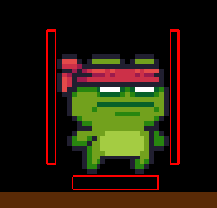
\includegraphics[width = 0.7\textwidth]{Imagenes/CollDetector.png}
	\caption{Representación de las cajas de detección de colisiones del jugador}
	\label{fig:Player_Coll_Detector}
\end{figure}

\textbf{Valores de configuración}
\begin{itemize}
	\item (bool) Debug Boxes: En caso de que esta variable sea true, las cajas definidas por los campos que serán presentandos a continuación serán representadas en pantalla con color rojo.
	\item (LayerMask) Detection Layers: Capas que serán tomadas en cuenta para detectar si el jugador está en el suelo o en contacto con una pared cuando está en el aire. En este caso se querrá especificar la capa que albergue a los objetos estáticos que conforman el mundo, por ejemplo \textit{World}.
	\item (Vector2) Bottom/Right/Left Size: Tamaño de las cajas.
	\item (Vector2) Bottom/Right/Left Offsets: Valores usados para reposicionar las cajas para que estén en el lugar considerado por el usuario, idealmente en los bordes del objeto.
\end{itemize}
\subsubsection{PlayerBetterJumping}

Para que el salto se ajuste más al estándar de los juegos de plataformas 2D, este script mejora la sensación de salto para que el personaje caiga más rápido, evitando una sensación de flotación. Además, permite realizar saltos más pequeños si el jugador suelta el botón antes.\\

Para lograrlo, el script ajusta dos multiplicadores: uno que incrementa la gravedad cuando el jugador está cayendo y otro que reduce la altura del salto cuando este es interrumpido antes de tiempo.\\

\textbf{Valores de configuración}
\begin{itemize}
	\item (float) Fall Multiplier: Multiplicador que aumenta la gravedad cuando el personaje está cayendo, hace que el personaje caiga más rapido, dándole más peso y realismo al salto.
	\item (float) Low Jump Multiplier: Multiplicador que aumenta la gravedad cuando el jugador suelta el botón de salto antes de llegar al punto más alto del salto haciendo que se puedan hacer saltos cortos dando más control del movimiento al jugador.
\end{itemize}
\subsection{Life}

Se ha implementado una clase Life que gestiona los puntos de salud del objeto al que está adjunto y que se encarga de eliminar el objeto en el caso que su vida llegue a cero. El componente pedirá al usuario un valor inicial para los puntos de vida del objeto y un valor máximo al que puede llegar la vida, para que esta sea limitada en caso de que se quiera implementar un sistema de recuperación de vida.\\

Este componente está estrechamente ligado al \textit{DamageSensor} el cual será mencionado más adelante y que detecta si ha habido una colisión con un objeto que aplique daño, esta relación es necesaria ya que para que se detecte el daño que decrementa la salud del objeto se necesita este sensor, por lo que al añadir un componente \textit{Life} se añadirá este sensor automáticamente.\\

\textit{Life} diferencia entre enemigos y el jugador, en caso de que el componente esté adjunto al jugador se deberá marcar en la opción \textit{EntityType} y el componente requerirá que se le de la referencia a un texto del \textit{Canvas} donde se escribirá la vida actual del jugador.\\

\textbf{Valores de configuración}
\begin{itemize}
	\item (enum) Entity Type: Enumerado usado para diferenciar entre jugador y enemigos.
	\item (float) Initial Life: Cantidad de vida con la que inicia la entidad.
	\item (float) Max Life: Cantidad de vida máxima a la que puede llegar la entidad.
	\item (string) Text Name: En caso de ser el jugador se pedirá un texto que precederá a los puntos de vida del jugador.
	\item (TextMeshProUGUI) Life Text: Objeto del Canvas usado para representar los puntos de vida actuales del jugador.
\end{itemize}

\subsection{PlayerDistanceAttack}

Componente encargado de representar un posible ataque a distancia del jugador. El ataque se activará con el clic izquierdo del ratón, lo que instanciará el prefab \textit{Bullet Prefab} en la posición del jugador (será importante que no el objeto instanciado no pueda colisionar con el jugador), el cual deberá albergar el comportamiento de una bala. La dirección que tomará la bala será aquella en la que se encuentre el cursor del ratón en el momento del clic.\\

Para evitar que el jugador pueda disparar sin restricción, se ha introducido un tiempo de espera entre disparos.\\

\textbf{Valores de configuración}
\begin{itemize}
	\item (GameObject) Bullet Prefab: Objeto que se instancia en la posición del jugador al hacer clic.
	\item (float) Shooting Cooldown: Tiempo necesario (en segundos) antes de poder disparar nuevamente.
\end{itemize}

\section {FSM}

El comportamiento de la entidad estará encapsulado en una FSM, cuya única funcionalidad es la de gestionar el estado actual, comprobar que no ha habido ningún cambio de estado y, en caso de haberlo, manejar el cambio de estado. Esta comprobación se hará al finalizar la actualización del estado actual (en el \texttt{LateUpdate}) para así evitar problemas con cambiar de estado en medio de un bucle sin terminar.\\

\textbf{Valores de configuración}
\begin{itemize}
	\item (State) Initial State: Estado inicial de la FSM.
\end{itemize}

\subsection{Transition}
Esta clase representa una transición de estado. Está compuesta por un sensor y un estado objetivo.\\

Si el sensor se activa, la entidad cambiará automáticamente al estado especificado.\\

\textbf{Valores de configuración}
\begin{itemize}
	\item (Sensor) Sensor: Sensor encargado de detectar el evento que hará que el cambio de estado se dé.
	\item (State) Target State: Estado de destino de la transición.
\end{itemize}

\subsection{State}

La clase \textit{State} representa un estado de comportamiento de un enemigo. Para ello gestiona dos elementos fundamentales: \textit{Actuators} y \textit{Sensors}.\\

\textbf{Valores de configuración}
\begin{itemize}
	\item (List<Actuator>) Actuator List: Lista de Actuator que son actualizados en cada bucle y representan acciones, se abordarán a continuación.
	\item (List<SensorStatePair>) Transition List: Lista de Transition que pueden ser activadas, lo que supone un cambio de estado al estado objetivo.
	\item (List<DamageEmitter>) Damage Emitter in State: Lista de DamageEmitter activos en el estado y que son los encargados de reportar daño.
	\item (bool) Debug State: Booleano utilizado para indicar si se quiere que los Actuators en \textit{Actuator List} y Sensores en \textit{Transition List} muestren información a través del Gizmos.
\end{itemize}
Cuando se produce un cambio de estado, todos los actuadores y sensores se detienen, y los sensores se desuscriben de todas las transiciones a los que estuvieran vinculados.\\

\section{Actuator}

Como se ha mencionado anteriormente, un actuator es el script encargado de ejecutar una acción, por lo que para cada tipo de acción existirá un actuator que la represente.
La clase \textit{Actuator} representa la clase base de la que heredarán todos los tipos de actuadores.
Esta clase abstracta contiene métodos para crear, destruir y actualizar cada actuador, así como un booleano que indica si el Actuador tiene la depuración activa o no.\\

\subsection{MovementActuator}
La clase \textit{Movement Actuator} que hereda de \textit{Actuator} se usa para todos aquellos actuadores que realizan una acción de movimiento. \\
\textbf{Valores de configuración}
\begin{itemize}
	\item (bool) Is Accelerated: bool que indica si el movimiento que se va realizar tiene una velocidad constante (valor a false), o que por el contrario, la velocidad va a ir variando (valor a true)
	\item (EasingFunction.Ease) Easing Function: Función que define el movimiento 
\end{itemize}

\subsubsection{HorizontalActuator}
\textit{Horizontal actuator}es un actuador que hereda de \textit{Movement Actuator} y permite mover un objeto horizontalmente, ya sea a la izquierda o a la derecha, con diferentes configuraciones de velocidad y comportamientos tras una colisión.\\
\textbf{Valores de configuración}
\begin{itemize}
	\item (LayerMask) Layers To Collide: mascara de capas que indica cuales son las que utilizamos para colisionar con el objeto.
	\item (enum) Direction: dirección inicial del movimiento. Puede ser \textit{Left} o \textit{Right}.
	\item (enum) On Collision Reaction: Reacción que va a tener el objeto al colisionar.Puede ser \textit{None} (sin reacción), \textit{Bounce} (rebota cambiando la dirección), o \textit{Destroy} (se destruye al colisionar).
	\item (float) Speed: Velocidad del movimiento
	\item (float) Goal Speed: Velocidad final del movimiento si este es acelerado.
	\item (float) Interpolation Time: Duración en segundos que va desde la velocidad inicial a \textit{ Goal Speed}
	\item (bool) Throw: Indica si el movimiento es un lanzamiento, es decir, si esá a true, se lanzará inicialmente con una velocidad inicial y, en caso contrario, seaplicará constantemente una fuerza.
	\item (bool) Follow Player: si es \textit{true}, la dirección del movimiento se ajusta automáticamente para acercarse al jugador.
\end{itemize}

\subsubsection{VerticalActuator}
\textit{Vertical actuator}es un actuador que hereda de \textit{Movement Actuator} y permite mover un objeto verticalmente, ya sea arriba o abajo, con diferentes configuraciones de velocidad y comportamientos tras una colisión.\\
\textbf{Valores de configuración}
\begin{itemize}
	\item (LayerMask) Layers To Collide: Mascara de capas que indica cuales son las que utilizamos para colisionar con el objeto.
	\item (enum) Direction: Dirección inicial del movimiento. Puede ser \textit{Up} o \textit{Down}.
	\item (enum) On Collision Reaction: Reacción que va a tener el objeto al colisionar.Puede ser \textit{None} (sin reacción), \textit{Bounce} (rebota cambiando la dirección), o \textit{Destroy} (se destruye al colisionar).
	\item (float) Speed: Velocidad del movimiento
	\item (float) Goal Speed: Velocidad final del movimiento si este es acelerado.
	\item (float) Interpolation Time: Duración en segundos que va desde la velocidad inicial a \textit{Goal Speed}
	\item (bool) Throw: Indica si el movimiento es un lanzamiento, es decir, si esá a true, se lanzará inicialmente con una velocidad inicial y, en caso contrario, seaplicará constantemente una fuerza.
	\item (bool) Follow Player: si es \textit{true}, la dirección del movimiento se ajusta automáticamente para acercarse al jugador.
\end{itemize}

\subsubsection{DirectionalActuator}
La clase \textit{Directional Actuator} que hereda de \textit{ Movement Actuator} se usa para describir un movimiento en función de un ángulo y una velocidad.\\
\textbf{Valores de configuración}
\begin{itemize}
	\item (LayerMask) Layers To Collide: capas con las que puede colisionar el objeto y activar reacciones.
	\item (float) Speed: Velocidad del movimiento
	\item (float) Goal Speed: Velocidad final del movimiento si este es acelerado.
	\item (float) Interpolation Time: Duración en segundos que va desde la velocidad inicial a \textit{Goal Speed}
	\item (float) Angle: Ángulo de dirección del movimiento, en grados.
	\item (bool) Throw:  Indica si el movimiento es un lanzamiento, es decir, si esá a true, se lanzará inicialmente con una velocidad inicial y, en caso contrario, seaplicará constantemente una fuerza.
	\item (enum) On Collision Reaction: Reacción que va a tener el objeto al colisionar.Puede ser \textit{None} (sin reacción), \textit{Bounce} (rebota cambiando la dirección), o \textit{Destroy} (se destruye al colisionar).
	\item (bool) Aim Player: Si es \textit{true}, el objeto calculará automáticamente el ángulo inicial para moverse en dirección al jugador.
\end{itemize}

\subsubsection{CircularActuator}
La clase \textit{Circular Actuator} que hereda de \textit{Movement Actuator} se usa para describir un movimiento circular alrededor de un punto.\\
\textbf{Valores de configuración}
\begin{itemize}
	\item (float) Angular Speed: Velocidad de giro en grados por segundos.
	\item (Transform) Rotation Point Position: Punto central de lacircunferencia  que describe el objeto.
	\item (float) Max Angle: Angulo máximo de giro. Si El ángulo es \textit{360º} entonces describirá una circunferencia completa, sino, hará un movimiento en forma de péndulo con los grados indicados. 
	\item (float) Angular Acceleration: Aceleración angular.
	\item (float) Goal Angular Speed: Velocidad angular que se quiere alcanzar si el objeto es acelerado.
	\item (bool) Can Rotate: si es \textit{true}, el objeto rota sobre sí mismo siguiendo la trayectoria.
	\item (float) Interpolation Time: tiempo en segundos que tarda desde la velocidad inicial hasta la velocidad final, \textit{Goal Speed}.
	\item (bool) Point Player: si es \textit{true}, el objeto ajusta su trayectoria para orientarse hacia el jugador.

\end{itemize}

\subsubsection{SplineActuator}
La clase \textit{Spline Actuator} que hereda de \textit{ Movement Actuator} se usa para describir un movimiento mediarte curvas Splines de Unity. El Actuador sigue la curva pudiendo girar el objeto a su vez.\\
\textbf{Valores de configuración}
\begin{itemize}
	\item (float) Speed: Velocidad del movimiento
	\item (float) Goal Speed: Velocidad final del movimiento si este es acelerado.
	\item (float) Interpolation Time: Duración en segundos que va desde la velocidad inicial a \textit{Goal Speed}
	\item (SplineContainer) Spline Container: Spline que define la trayectoria que seguirá el objeto.
	\item (enum) Teleport To Closest Point: Define cómo se ajusta el objeto a la spline al iniciarse el movimiento. Puede tener dos valores:
	\begin{itemize}
		\item \textbf{Enemy}: el objeto se teletransporta a la spline.
		\item \textbf{Spline}: la spline se desplaza para alinearse con la posición actual del objeto.
	\end{itemize}
\end{itemize}

\subsubsection{MoveToAPointActuator}
La clase \textit{Move to a Point Actuator} que hereda de \textit{ Movement Actuator} se usa para mover el objeto en  dirección a un punto no actualizable. Puede ser a un punto concreto y seguir una lista de ellos o a puntos aleatorios desntro de un área.\\
\textbf{Valores de configuración}
\begin{itemize} 
	\item (UsageWay) Usage Way: Define si se va a seguir una ruta por puntos (\textit{Waypoint}) o si se escogen puntos aleatoriamente dentro de una zona  (\textit{RandomArea}).
	\item (List<WaypointData>) Waypoints Data: lista de puntos que el objeto debe seguir. Cada punto incluye el tiempo que se tarda en llegar, si se desea aceleración, si se debe detener al llegar, duración de la parada y función de aceleración si es necesaria. 		
	
	 \item (Collider2D) Random Area: Zona dentro de la cual se moverá el objeto si está configurado como \textit{RandomArea}. 
	\item (bool) Is a Cicle: si es true, al finalizar los puntos volverá al primero y el movimiento se repetirá. 
	\item (bool) All Waypoints Have The Same Data: si es true, todos los puntos usarán la misma configuración. 
\end{itemize}

\subsubsection{MoveToAnObjectActuator}
La clase \textit{Move to an Object Actuator} que hereda de \textit{Movement Actuator} se usa para mover el objeto en  dirección a un punto actualizable, esto implica que si el punto se muve, el objeto actualizará la trayectoria a la nueva posición. \\
\textbf{Valores de configuración}
\begin{itemize} 
	\item (UsageWay) Usage Way: Define si se va a seguir una ruta por puntos (\textit{Waypoint}) o si se escogen puntos aleatoriamente dentro de una zona  (\textit{RandomArea}).
	\item (List<WaypointData>) Waypoints Data: lista de puntos que el objeto debe seguir. Cada punto incluye el tiempo que se tarda en llegar, si se desea aceleración, si se debe detener al llegar, duración de la parada y función de aceleración si es necesaria. 		
	
	 \item (Collider2D) Random Area: Zona dentro de la cual se moverá el objeto si está configurado como \textit{RandomArea}. 
	\item (bool) Is a Cicle: si es true, al finalizar los puntos volverá al primero y el movimiento se repetirá. 
	\item (bool) All Waypoints Have The Same Data: si es true, todos los puntos usarán la misma configuración. 
\end{itemize}

\subsection{SpawnerActuator}
La clase \textit{SpawnerActuator} hereda de \textit{Actuator}. Este actuador se usa para poder generar nuevos enemigos. Pudiendo generar infinitos enemigos o un numero definido de ellos cada X tiempo en un lugar predefinido.

\textbf{Valores de configuración}
\begin{itemize}
    \item (class) \textbf{Spawn Info}: Clase auxiliar serializable que almacena un prefab (\texttt{GameObject}) a instanciar y un punto de aparición (\texttt{Transform}) donde se colocará dicho objeto.
    \item (float) \textbf{ Spawn Interval}: Intervalo de tiempo en segundos que tarda el objeto en volver a generar otro enemigo. 
    \item (bool) \textbf{Infinite Enemies}: Indica si se generarán enemigo indefinidamente. Si es verdadero, se crearán continuamente nuevos enemigos cada X tiempo indicado por  \textit{spawnInterval}  y si es falso, el número de spawns estará limitado por \texttt{Number of Times To Spawn}.
    \item (int) \textbf{Number of Times To Spawn}: Número total de veces que se permitirá hacer spawn, si no es infinito.
    \item (List<SpawnInfo>) \textbf{Spawn List}: Lista de elementos de tipo \texttt{Spawn Info}. Cada elemento contiene la información necesaria para instaciar un enemigo. Esta lista está diseñada para poder crear distintos tipos de enemigos o en varios sitios a la vez, dando así más flexibilidad.
\end{itemize}


\section{Sensors and Emitters}

Para que exista una comunicación entre la entidad y su entorno, esta necesita poder recibir y enviar información. Con este propósito se diseñan los sensores y los emisores.\\

\subsection{Sensor}

La clase \textit{Sensor} es de la que heredarán los sensores utilizados en la herramienta. Esta clase contiene variables como el evento que almacena las funciones que se deberán de llamar en caso de que el sensor sea activado, como puede ser la función que activará la transición posteriormente.\\

Cualquier clase que herede de \textit{Sensor} tendrá la posibilidad de modificar tres funciones relativa a la lógica del sensor:

\begin{itemize}
	\item \texttt{StartSensor}: Función que se encargada de activar el sensor para que se pueda comenzar a captar información y en caso de querer un tiempo de espera al inicio de la activación, se crea el \textit{timer} correspondente.
	\item \texttt{UpdateSensor}: Función llamada en cada bucle y encargada de actualizar el tiempo que queda por esperar en caso de que el \textit{timer} no haya acabado.
	\item \texttt{StopSensor}: Función que desactiva el sensor.
\end{itemize}
Estas funciones son las encargadas de gestionar las variables de control.

En caso de que se quiera agregar lógica extra a alguna de estas funciones para un sensor en específico, se puede sobreescribir estos métodos en la clase del sensor correspondiente con la condición de que es indispensable que se llame al método de la clase base.
\comp{Foto del código?}

También se incluye un modo debug opcional, activable mediante el método \texttt{SetDebug(bool)}, método que será llamado desde State y tomará el valor de la variable \textit{Debug State} del propio estado.\\

La funcionalidad de los sensores se ha implementado de manera que si se quiere suscribir desde un componente a un evento de cualquier sensor se podrá hacer siempre y cuando la función que será llamada en caso de activarse el sensor reciba un objeto de tipo \textit{Sensor}.\\

\comp{Veo la explicación confusa y con una imagen sería más claro, es raro poner una imagen de un trozo de código? Entiendo que sí.}

La implementación del evento incluye un contador de suscriptores que permite llevar un control interno sobre cuántos componentes están actualmente registrados para recibir notificaciones del sensor. Esta es una práctica útil para evitar errores en tiempo de ejecución.\\

Es importante tener en cuenta que toda suscripción a un sensor debe ir acompañada, en algún momento, de su correspondiente desuscripción. Un caso típico es realizar esta desuscripción cuando la entidad es destruida, utilizando el método \texttt{OnDestroy}.\\

\textbf{Valores de configuración}
\begin{itemize}
	\item (float) Start Detecting Time: Tiempo que necesitará el sensor para activarse al entrar en el estado que lo alberga.
\end{itemize}


A continuación se enumerarán y explicarán los tipos de sensores incluidos en la herramienta.\\
\subsubsection{AreaSensor}

\textit{AreaSensor} representa un tipo de sensor espacial que detecta la presencia de un objeto objetivo dentro de una zona delimitada. Está pensado para funcionar con zonas de activación, por lo que requiere que el objeto que lo contiene tenga un componente \textit{Collider2D}. Esta condición se asegura mediante el atributo \texttt{[RequireComponent(typeof(Collider2D))]}, que obliga a Unity a añadir automáticamente ese componente si no está presente.\\

La detección se realiza mediante los métodos \texttt{OnTriggerEnter2D} y \texttt{OnTriggerStay2D} provistos por \textit{Unity}. El primero detecta la entrada del objetivo en la zona, mientras que el segundo permite capturar situaciones en las que el objetivo ya se encuentra dentro del área al momento de activarse el sensor. Esto evita perder eventos relevantes si la detección no estaba habilitada previamente.\\

Al usarse métodos como \texttt{OnTriggerEnter2D} y \texttt{OnTriggerStay2D} se activará automáticamente la flag que convierte un \textit{Collider2D} en un trigger.\\

\textbf{Valores de configuración}
\begin{itemize}
	\item (GameObject) Target: Objeto que se quiere detectar dentro de la zona delimitada por el Collider2D.
\end{itemize}

\subsubsection{CollisionSensor}

\textit{CollisionSensor} es el sensor encargado de detectar la colisión de un objeto con un grupo determinado de objetos.\\

Al igual que en \textit{AreaSensor}, se necesitará un \textit{Collider2D} para detectar colisiones y se obligará a Unity a añadirlo de la misma manera.\\

Para acotar con que objetos se activa el sensor y con cuales no, se utilizarán las \textit{LayerMask} de \textit{Unity} y se detectarán las colisiones con \texttt{OnCollisionEnter2D} y \texttt{OnCollisionStay2D}, por lo que para reportar una colisión ninguno de los dos objetos deben ser trigger.\\

\textbf{Valores de configuración}
\begin{itemize}
	\item (LayerMask) Layers To Collide: Máscara de capas físicas que, en caso de colisión, activarán el sensor.
\end{itemize}

\subsubsection{DamageSensor}

\textit{DamageSensor} es un tipo de sensor que detecta las colisiones y entradas en el área de un objeto que emite daño. Este sensor está diseñado para funcionar tanto con colisiones como con triggers. Requiere que el objeto al que se le asigne tenga un componente \textit{Collider2D}, lo cual se asegura automáticamente gracias al atributo \texttt{[RequireComponent(typeof(Collider2D))]}.\\

La funcionalidad de este sensor es doble. Además de activar transiciones, se utiliza para gestionar la lógica del componente \textit{Life}. En caso de colisión, y bajo ciertas condiciones, como colisionar con un objeto que tenga el componente \textit{DamageEmitter}, el sensor se activa. Luego, desde el componente \textit{Life}, se gestiona qué hacer en función de las características del \textit{DamageEmitter}.\\

El sensor puede ser configurado para que se active desde el inicio mediante el atributo \textit{Active From Start}, lo que permite que el sensor sea útil en caso de que no se quiera que el sensor esté implicado en ninguna transición, pero si en el sistema de gestión de salud.\\

El sensor detecta las entradas y salidas de objetos mediante los métodos \texttt{OnTriggerEnter2D}, \texttt{OnTriggerExit2D}, \texttt{OnCollisionEnter2D} y \texttt{OnCollisionExit2D}. Este control será necesario para gestionar los distintos tipos de daños que serán abordados más adelante.\\

\textbf{Valores de configuración}
\begin{itemize}
	\item (bool) Active From Start: Si es verdadero, el \textit{DamageSensor} no tendrá porqué ser incluido en ninguna transición para que este se considere activo.
\end{itemize}

\subsubsection{DistanceSensor}

\textit{DistanceSensor} es el sensor utilizado para medir la distancia entre dos puntos. La distancia se medirá tomando de referencia los \textit{Transform} de sendos objetos, uno de ellos el que posee este script y el otro el objetivo de la medición.\\

El funcionamiento del sensor dependerá del valor asignado a la variable \textit{Distance Type}, la cual es de un tipo enumerado \textit{TypeOfDistance} que especifica la manera en que se calculará la distancia. Según el valor de esta variable, se requerirán distintos parámetros o configuraciones, aunque varios valores de configuración seguirán siendo necesarios independientemente de \textit{Distance Type}.\\

\textbf{Valores de configuración comunes}
\begin{itemize}
	\item (enum) Distance Type: Tipo enumerado que determinará de que manera se mide la distancia y que variables se necesitarán para medirla.
	\item (enum) Detection Condition: Tipo enumerado que determina si el sensor se activa cuando el objetivo está dentro de esa distancia o cuando está fuera de la misma.
	\item (GameObject) Target: Entidad con la que se mide la distancia.
\end{itemize}

A continuación se especificarán los valores que puede tomar el enumerado \textit{TypeOfDistance} y las variables específicas necesarias en cada caso.\\

\textbf{Valores de \textit{TypeOfDistance}}

\begin{itemize}
	\item \textit{Area}

Creo que esto está mal ya que hace el mismo trabajo que el Sensor de Area.

\textbf{Valores de configuración}
	\begin{itemize}
	        \item A
	 \end{itemize
}
	\item \textit{Magnitude}

	Configuración utilizada cuando se quiere medir la distancia como magnitud. La representación gráfica de esta forma de medir la distancia es un círculo, como se muestra en la \autoref{fig:DistanceSensor_Magnitude}.\\
Dependiendo del valor de la variable \textit{Detection Condition} el sensor se activará si el objeto objetivo está dentro o fuera del círculo.
	\begin{figure}[t]
		\centering
		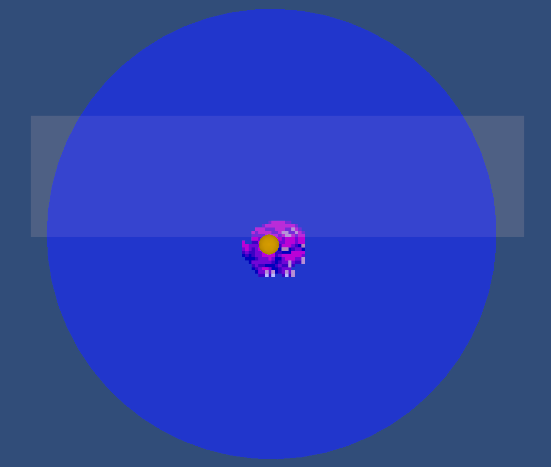
\includegraphics[width = 0.7\textwidth]{Imagenes/DistanceSensorMagnitude.png}
		\caption{Medición de distancia a través de la magnitud.}
		\label{fig:DistanceSensor_Magnitude}
	\end{figure}

	\textbf{Valores de configuración}
	\begin{itemize}
	        \item (float) Detection Distance: Distancia necesaria para que el sensor se active.
	 \end{itemize}

	\item \textit{Single Axis}

Con el tipo de medida \textit{Single Axis} se mide la distancia entre ambos objetos pero solo en uno de los dos ejes: X o Y.\\

	\textbf{Valores de configuración}
	\begin{itemize}
	        \item (float) Detection Distance: Distancia necesaria para que el sensor se active.
	        \item (enum) Axis: Da opciones para escoger cual de los dos ejes se va a medir, si X o Y.
	        \item (enum) Detection Sides: Permite elegir si se quiere medir la distancia a ambos lados del eje o solo por uno de ellos. 
	        \item (enum) Part: En caso de que se haya determinado que solo se quiere medir la distancia en uno de los dos lados del eje elegido se deberá especificar cual de los dos es. Por ejemplo si queremos medir la distancia en el eje X, nos permite medir cuando el objetivo entra en el rango determinado por \textit{Detection Distance} por la izquierda o por la derecha.
	 \end{itemize}
\end{itemize}


\subsubsection{TimeSensor}

Sensor encargado de activarse cuando pasa un tiempo determinado desde su activación.\\
En caso de ajustar que el sensor necesitará un tiempo de activación, primero se procederá a medir tal tiempo y cuando este llegue a su fin, se medirá el tiempo de activación propio del sensor.\\

\textbf{Valores de configuración}
	\begin{itemize}
	        \item (float) Detection Time: Tiempo necesario, medido en segundos, para que el sensor se active.
	 \end{itemize}

\subsection{DamageEmitter}

Para que una entidad pueda emitir daño, debe tener adjunto el componente \textit{DamageEmitter}.\\
Este componente no implementa funcionalidad adicional en su propio script, sino que actúa como una señal para el \textit{DamageSensor}. La detección de daño por parte del sensor depende de que el objeto con el que colisiona tenga este componente adjunto.\\

La manera en la que \textit{DamageEmitter} reporta daño dependerá de un tipo enumerado llamado \textit{DamageType}.\\
Como valores de configuración comunes para todas las configuraciones disponibles encontramos.\\

\textbf{Valores de configuración comunes}
\begin{itemize}
	\item (bool) Active From Start: En caso de que esté desactivado, no se reportará daño a no ser que el \textit{DamageEmitter} esté incluido en un estado.
	\item (enum) Damage Type: Diferentes formas de producir daño a las entidades que tengan \textit{DamageSensor}.
\end{itemize}

A continuación se concretarán los valores que puede tomar el enumerado \textit{DamageType}, como funciona cada tipo de daño y que otros valores de configuración serán necesarios.\\

\textbf{Valores de \textit{DamageType}}

\begin{itemize}
	\item \textit{Instant}
Tipo de daño que se aplica una vez producido el contacto y que no se va a volver a aplicar hasta que ese contacto no haya finalizado y se de uno nuevo.\\

\textbf{Valores de configuración}
	\begin{itemize}
	        \item (bool) Destroy After Doing Damage: Booleano que determina si el objeto es destruido al reportar daño.
	        \item (bool) Instant Kill: Determina si la entidad que reporta daño elimina a su objetivo instantáneamente.
	        \item (float) Damage Amount: En caso de no eliminar instantáneamente al objetivo, se especificará la cantidad de daño que se hará.
	 \end{itemize}
	\item \textit{Persistent}
El daño persistente es aquel que produce constántemente una entidad cada X tiempo. Este daño se producirá mientras dure la colisión o, en caso de que sea un trigger, la superposición.\\

\textbf{Valores de configuración}
	\begin{itemize}
	        \item (float) Damage Amount: Cantidad de daño administrada cada vez.
	        \item (float) Damage Cooldown: Tiempo necesario para administrar daño de nuevo, medido en segundos.
	\end{itemize}

	\item \textit{Residual}
El daño residual es aquel que produce una cantidad de daño instantáneo y tras esto produce un número determinado de aplicaciones de otra cantidad de daño cada cierto tiempo.\\

\textbf{Valores de configuración}
	\begin{itemize}
	        \item (bool) Destroy After Doing Damage: Booleano que determina si el objeto es destruido al reportar el daño instantáneo.
	        \item (float) Instant Damage Amount: Cantidad de daño administrada cuando se produce el contacto.
	        \item (float) Residual Damage Amount: Cantidad de daño administrada por cada aplicación de daño residual.
	        \item (float) Damage Cooldown: Tiempo entre aplicaciones de daño residual, medido en segundos.
	        \item (int) Number Of Applications: Número de veces que se aplicará el daño residual.
	\end{itemize}
\end{itemize}

\section{Animations}
La clase \textit{AnimatorManager} se encarga de gestionar las animaciones de cada enemigo, en función del movimieno, es decir de los actuadores que esten activos.\\

\textbf{Valores de configuración}
\begin{itemize}
	\item (bool) Can Flip X: Indica si el sprite puede voltearse horizontalmente.
	\item (bool) Can Flip Y: Indica si el sprite puede voltearse verticalmente. 
\item (SpriteRender) Sprite Render: Referencia al Sprite Render del propio objeto.
\end{itemize}

Durante la ejecución, se actualizan continuamente los parámetros \textit{XSpeed},  \textit{YSpeed}  y  \textit{RotationSpeed}  del animator a partir de la velocidad del \textit{Rigidbody2D}, lo que permite que las animaciones reflejen con precisión el movimiento real del objeto. Además, si el enemigo cambia de dirección, los sprites rotarán siempreque se hayan activado  los booleanos previamente mencionados.

Cuando el enemigo recibe daño o muere, se activan los triggers \textit{Damage} y \textit{Die} respectivamente, lo que lanza las animaciones correspondientes. En el caso de la muerte, el objeto se destruye automáticamente una vez finaliza la animación. 

Por otro lado, la clase permite cambiar indicar si el enemigo está siguiendo a otro objeto con el parámetro \textit{Follow} o saber si la FSM ha cambiado de estadofunción \textit{ChangeState}.

Finalmente, al invocar eventos de aparición, se activa el trigger \textit{Spawn}.

\textbf{Parámetros requeridos en el Animator}
\begin{itemize}
	\item Triggers: \textit{Die}, \textit{Damage}, \textit{Spawn}, \textit{ChangeState}
	\item Bools: \textit{Left}, \textit{Right}, \textit{Up}, \textit{Down}, \textit{Follow}, \textit{Rotating}
	\item Floats: \textit{XSpeed}, \textit{YSpeed}, \textit{RotationSpeed}
\end{itemize}
Para facilitar la gestión de los estados y de los parámetros del Animator, se ha creado un controlador  \textit{Controller} que pretende servir de base para la gestión de las animaciones.


